%%%%%%%%%%%%%%%%%%%%%%%%%%%%%%%%%%%%%%%%%%%%%%%%%%%%%%%%%%%%%%%%%%
%%%%%%%%%%%%%%%%%%%%%%%%%%%%%%%%%%%%%%%%%%%%%%%%%%%%%%%%%%%%%%%%%%
%Packages
\documentclass[10pt, a4paper]{article}
\usepackage[top=3cm, bottom=4cm, left=3.5cm, right=3.5cm]{geometry}
\usepackage{amsmath,amsthm,amsfonts,amssymb,amscd, fancyhdr, color, comment, graphicx, environ}
\usepackage{float}
\usepackage{mathrsfs}
\usepackage[math-style=ISO]{unicode-math}
\setmathfont{Calibri}
\usepackage{lastpage}
\usepackage[dvipsnames]{xcolor}
\usepackage[framemethod=TikZ]{mdframed}
\usepackage{enumerate}
\usepackage[shortlabels]{enumitem}
\usepackage{fancyhdr}
\usepackage{indentfirst}
\usepackage{listings}
\usepackage{sectsty}
\usepackage{thmtools}
\usepackage{shadethm}
\usepackage{hyperref}
\usepackage{setspace}
\usepackage{biblatex}
\usepackage{csvsimple}
\usepackage{amsmath}
\usepackage{fontspec}
\usepackage{adjustbox}
\newfontfamily\faFont[Script=Arabic]{Calibri}   
\usepackage{bidi}
\newenvironment{Fa}{\begin{RTL}\faFont}{\end{RTL}}
\newcommand{\fa}[1]{{\faFont\RL{#1}}}
\hypersetup{
    colorlinks=true,
    linkcolor=blue,
    filecolor=magenta,      
    urlcolor=blue,
}
%%%%%%%%%%%%%%%%%%%%%%%%%%%%%%%%%%%%%%%%%%%%%%%%%%%%%%%%%%%%%%%%%%
%%%%%%%%%%%%%%%%%%%%%%%%%%%%%%%%%%%%%%%%%%%%%%%%%%%%%%%%%%%%%%%%%%
%Environment setup
\mdfsetup{skipabove=\topskip,skipbelow=\topskip}
\newrobustcmd\ExampleText{%
An \textit{inhomogeneous linear} differential equation has the form
\begin{align}
L[v ] = f,
\end{align}
where $L$ is a linear differential operator, $v$ is the dependent
variable, and $f$ is a given non−zero function of the independent
variables alone.
}
\mdfdefinestyle{theoremstyle}{%
linecolor=black,linewidth=1pt,%
frametitlerule=true,%
frametitlebackgroundcolor=gray!20,
innertopmargin=\topskip,
}
\mdtheorem[style=theoremstyle]{Problem}{Problem}
\newenvironment{Solution}{\textbf{Solution.}}

\definecolor{codegreen}{rgb}{0,0.6,0}
\definecolor{codegray}{rgb}{0.5,0.5,0.5}
\definecolor{codepurple}{rgb}{0.58,0,0.82}
\definecolor{backcolour}{rgb}{0.95,0.95,0.92}

\lstdefinestyle{mystyle}{
    backgroundcolor=\color{backcolour},   
    commentstyle=\color{codegreen},
    keywordstyle=\color{magenta},
    numberstyle=\tiny\color{codegray},
    stringstyle=\color{codepurple},
    basicstyle=\ttfamily\footnotesize,
    breakatwhitespace=false,         
    breaklines=true,                 
    captionpos=b,                    
    keepspaces=true,                 
    numbers=left,                    
    numbersep=5pt,                  
    showspaces=false,                
    showstringspaces=false,
    showtabs=false,                  
    tabsize=2
}

\lstset{style=mystyle}
%%%%%%%%%%%%%%%%%%%%%%%%%%%%%%%%%%%%%%%%%%%%%%%%%%%%%%%%%%%%%%%%%%
%%%%%%%%%%%%%%%%%%%%%%%%%%%%%%%%%%%%%%%%%%%%%%%%%%%%%%%%%%%%%%%%%%
%Fill in the appropriate information below
\newcommand{\norm}[1]{\left\lVert#1\right\rVert}     
\newcommand\course{NLP}                            % <-- course name   
\newcommand\hwnumber{1}                                 % <-- homework number
\newcommand\Information{Mohammadjavad Mehditabar - 98522049}                        % <-- personal information
%%%%%%%%%%%%%%%%%%%%%%%%%%%%%%%%%%%%%%%%%%%%%%%%%%%%%%%%%%%%%%%%%%
%%%%%%%%%%%%%%%%%%%%%%%%%%%%%%%%%%%%%%%%%%%%%%%%%%%%%%%%%%%%%%%%%%
%Page setup
\pagestyle{fancy}
\headheight 35pt
\lhead{\today}
\rhead{
\includegraphics[width=1cm]{images/iust-logo.png}}
\lfoot{}
\pagenumbering{arabic}
\cfoot{\small\thepage}
\rfoot{}
\headsep 1.2em
\renewcommand{\baselinestretch}{1.25}
%%%%%%%%%%%%%%%%%%%%%%%%%%%%%%%%%%%%%%%%%%%%%%%%%%%%%%%%%%%%%%%%%%
%%%%%%%%%%%%%%%%%%%%%%%%%%%%%%%%%%%%%%%%%%%%%%%%%%%%%%%%%%%%%%%%%%
%Add new commands here
% \renewcommand{\labelenumi}{\alph{enumi})}
\newcommand{\Z}{\mathbb Z}
\newcommand{\R}{\mathbb R}
\newcommand{\Q}{\mathbb Q}
\newcommand{\NN}{\mathbb N}
\newcommand{\PP}{\mathbb P}
\DeclareMathOperator{\Mod}{Mod} 
\renewcommand\lstlistingname{Algorithm}
\renewcommand\lstlistlistingname{Algorithms}
\def\lstlistingautorefname{Alg.}
\newtheorem*{theorem}{Theorem}
\newtheorem*{lemma}{Lemma}
\newtheorem{case}{Case}
\newcommand{\assign}{:=}
\newcommand{\infixiff}{\text{ iff }}
\newcommand{\nobracket}{}
\newcommand{\backassign}{=:}
\newcommand{\tmmathbf}[1]{\ensuremath{\boldsymbol{#1}}}
\newcommand{\tmop}[1]{\ensuremath{\operatorname{#1}}}
\newcommand{\tmtextbf}[1]{\text{{\bfseries{#1}}}}
\newcommand{\tmtextit}[1]{\text{{\itshape{#1}}}}

\newenvironment{itemizedot}{\begin{itemize} \renewcommand{\labelitemi}{$\bullet$}\renewcommand{\labelitemii}{$\bullet$}\renewcommand{\labelitemiii}{$\bullet$}\renewcommand{\labelitemiv}{$\bullet$}}{\end{itemize}}
\catcode`\<=\active \def<{
\fontencoding{T1}\selectfont\symbol{60}\fontencoding{\encodingdefault}}
\catcode`\>=\active \def>{
\fontencoding{T1}\selectfont\symbol{62}\fontencoding{\encodingdefault}}
\catcode`\<=\active \def<{
\fontencoding{T1}\selectfont\symbol{60}\fontencoding{\encodingdefault}}

%%%%%%%%%%%%%%%%%%%%%%%%%%%%%%%%%%%%%%%%%%%%%%%%%%%%%%%%%%%%%%%%%%
%%%%%%%%%%%%%%%%%%%%%%%%%%%%%%%%%%%%%%%%%%%%%%%%%%%%%%%%%%%%%%%%%%
%Begin now!



\begin{document}

\begin{titlepage}
    \begin{center}
        \vspace*{3cm}

        \Huge
        \textbf{Personality Detection on Persian Dataset}

        \vspace{1cm}
        \huge
        Phase \hwnumber

        \vspace{1.5cm}
        \Large

        \textbf{\Information}                      % <-- author


        \vfill

        \course \ Phase \hwnumber

        \vspace{1cm}

        
\includegraphics[width=0.4\textwidth]{images/iust-logo.png}
        \\

        \Large

        \today

    \end{center}
\end{titlepage}

%%%%%%%%%%%%%%%%%%%%%%%%%%%%%%%%%%%%%%%%%%%%%%%%%%%%%%%%%%%%%%%%%%
%%%%%%%%%%%%%%%%%%%%%%%%%%%%%%%%%%%%%%%%%%%%%%%%%%%%%%%%%%%%%%%%%%
%Start the assignment now
%%%%%%%%%%%%%%%%%%%%%%%%%%%%%%%%%%%%%%%%%%%%%%%%%%%%%%%%%%%%%%%%%%
%New problem
\newpage

\vspace*{0.1cm}

\tableofcontents

\newpage
% \vspace*{1pt}
\section{Data Overview}
Due to the lack of Persian datasets in the personality detection
field, gathering data from an adequate source is the main part of
our research. We came up with the idea of collecting data from
publicly available sources, thanks to social media, which is the best
and most applicable source. Because it contains a variety of people
and has a wide range of data, which is useful for us to collect. As a
result, we decided to choose Twitter as our data origin due to its
popularity, accessibility, and also comprise a lot of texts. We have
reached three different methods of collecting data

\section{Data Processing}

\subsection{Bio Search}

this dataset contains Iranian users with specified MBTI type of themselves in their bio.
There were some difficulties in distinguishing the language of some bios.
Hence they were solved by manual checking and some consideration of the Persian language.
Labels of this data are based on mentioned types in their bio, which we recognized by searching 16 MBTI types in their bio and automatically detecting them.
\\
This dataset consists of users' publicly available tweets and MBTI labels.
Figure \ref{bio_figure} shows a sample of our collected data based on a mentioned MBTI type on their bio.
\begin{figure}[h]
    \centering
    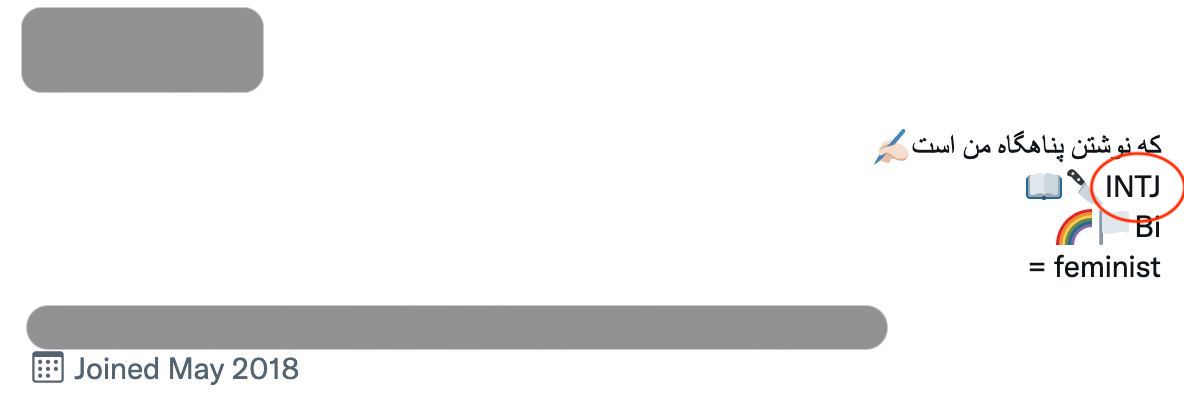
\includegraphics[width=.95\columnwidth]{images/sample.jpg}
    \caption{A sample of bio search}
    \label{bio_figure}
\end{figure}


\subsection{Tweet Search}
In this method, we tried collecting user tweets using a Python library called Twint.
Through this approach, we have searched for 16 possible MBTI labels in users' tweets in which one of these labels is mentioned.
Note that queried tweets are based on recent tweets in the Persian language.
We noticed that The type users mentioned in their tweets, may be irrelevant to themselves,
or they're saying some fact about this personality type or mentioning someone else's type.
Moreover, after filtering those users, we performed some elimination in a total separate step for the users
who have assigned themselves to multiple MBTI types. So these users are absolutely invalid for our dataset.
Hence there are chances that auto labeling makes a mistake in finding the correct label,
thus users are labeled manually so that ambiguity will be resolved.
\\
This dataset contains the gender of the user besides their tweets and MBTI label.
Figure \ref{tweet_figure} shows a sample of our collected data based on a mentioned MBTI type on their tweet.

\begin{figure}[h]
    \centering
    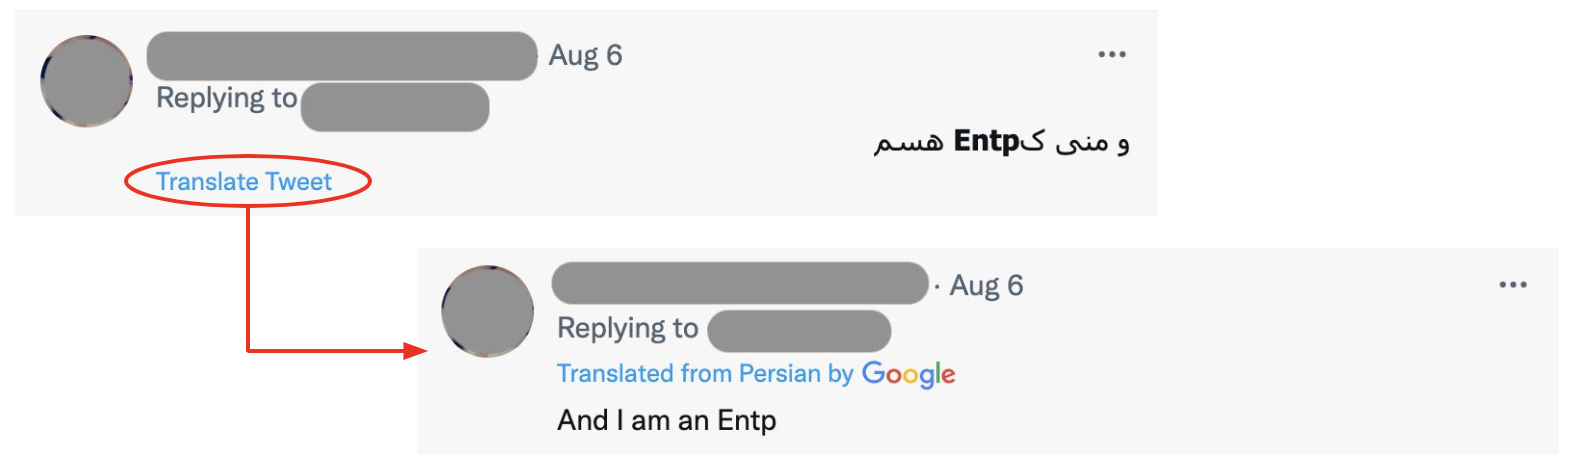
\includegraphics[width=.95\columnwidth]{images/sample-tweet.png}
    \caption{A sample of tweet search}
    \label{tweet_figure}
\end{figure}

\subsection{Questionnaire}
As our last method, we used a questionnaire to obtain more accurate data.
We can consider this data as the golden data.
The questionnaire was implemented in a web platform service with 60 standard well-known MBTI tests in which users
filled their Twitter IDs and answered those questions. We received a
few more data from users as well as their gender, location, degree of education,
and age for analyzing and adding more features to our data to perform well on the dataset.
Labeling them was based on their answer and how close they were to each of four binary class types (i.e. I/E, S/N, T/F, P/J),
which were calculated after completing the questionnaire.
Tweets of them are collected by the Python library Tweepy, which is a helpful tool to gain all their tweets.
Users are verified through the unique token generated for each user.
With this technique, we'll prevent fake data from entering our dataset.
Also, we filtered users to have at least 150 tweets, and their account is public.
Our questionnaire was utterly ethical since all users completed it voluntarily, and their account was public.

\subsection{Data Cleaning}
We follow a relatively straightforward strategy to clean our textual data.
Firstly, we find and replace some special patterns with unique tokens using regular expressions.
More specifically, we replace URLs with [LINK], usernames with [USERNAME], emojis with [EMOJI], and smileys with [SMILEY].
We also take a step further to filter out non-Persian characters.
For this purpose, we carefully select specific ranges of the Unicode characters to be allowed in our data.
We find that this step substantially improves the performance of our models.
Finally, we only preserve users that have more than 100 tweets after performing the above-mentioned cleanings.
\\
Also I should mention that, we used another approach which is cleaning more agressively. In this method we remove any non-Persian
characters and all tweets are splitted with just space, not any other punctuation marks.


\newpage
\subsubsection*{The following will give you an overview of what you can do with this template.}

\begin{Problem}
    Type your problem here. \\

    Personally I recommend Mathpix (https://mathpix.com/), which can easily export your ProblemBook.pdf to \LaTeX \ code.
\end{Problem}

\begin{Solution}
    Write your solution here.

    Example of equations. $x+1=2$. Or
    $$x-1=0$$

    Example of a list of equations.
    \begin{align*}
        x & = 1 \\
        y & = 2
    \end{align*}

    Example of a matrix.
    $$\begin{pmatrix}1&0\\0&1\end{pmatrix}$$

    Example of a lemma.
    \begin{lemma}
        This is a lemma.
    \end{lemma}

    \section{coda explaination}

    \begin{Fa}
        پاراگراف فارسی
        ممد اومد انجیا
        sda
        منم منم منن
        چطوری پسر
        sad
        ستون
        سلام
        میو میو


        \centering
        \begin{adjustbox}{center}

            \csvautotabular{../stats/RNF.csv}
        \end{adjustbox}

        % \end{align*}
    \end{Fa}
    This is a Persian word: \fa{سیب}. It means apple. so what

    Example of a proof.
    \begin{proof}
        Write your proof here.
    \end{proof}

    Example of including a picture.
    \begin{center}
        
\includegraphics[width = 4cm]{logo-hkust.png}
    \end{center}

    Example of referring to a piece of code.
    my main problem is \(what the hell\) is something happening
    \lstinputlisting[language = python]{Program Solution.py}

    Example of a table.
    \begin{equation*}\begin{tabular}{ c c c }
                      & Mean     & SD       \\
            Fall 2077 & 7.046512 & 1.714552 \\
            Fall 1977 & 9.102941 & 1.568919
        \end{tabular}\end{equation*}

    Overall, this is a quite basic template for assignments, and above are only some basic features. I included enough packages and set a few environments. You may modify them or add features to fit your personal preference. Enjoy using it!
\end{Solution}

%%%%%%%%%%%%%%%%%%%%%%%%%%%%%%%%%%%%%%%%%%%%%%%%%%%%%%%%%%%%%%%%%%
%Complete the assignment now
\end{document}

%%%%%%%%%%%%%%%%%%%%%%%%%%%%%%%%%%%%%%%%%%%%%%%%%%%%%%%%%%%%%%%%%%
%%%%%%%%%%%%%%%%%%%%%%%%%%%%%%%%%%%%%%%%%%%%%%%%%%%%%%%%%%%%%%%%%%
